% !TeX root = ../main.tex

\chapter{ATLAS 探测器}
ATLAS 探测器是大型强子对撞机(Large Hadron Collider,LHC)上的一个探测器,它拥有对于对撞中心接近全空间立体角的探测范围。
ATLAS 探测器是一个多用途探测器,由一个被薄超导螺线管包围的内部径迹探测器、电磁和强子量能器以及一个包含三个大型超导环形磁体的μ子谱仪组成,
其剖面图见\autoref{fig:ATLAS_Drawing_with_Labels}。
内部探测器系统处于 2 T 轴向磁场中,拥有 $\abs{\eta} < 2.5$ 范围内带电粒子径迹探测能力。
\cite{ATLAS_detector}

\begin{figure}[ht]
    \centering
    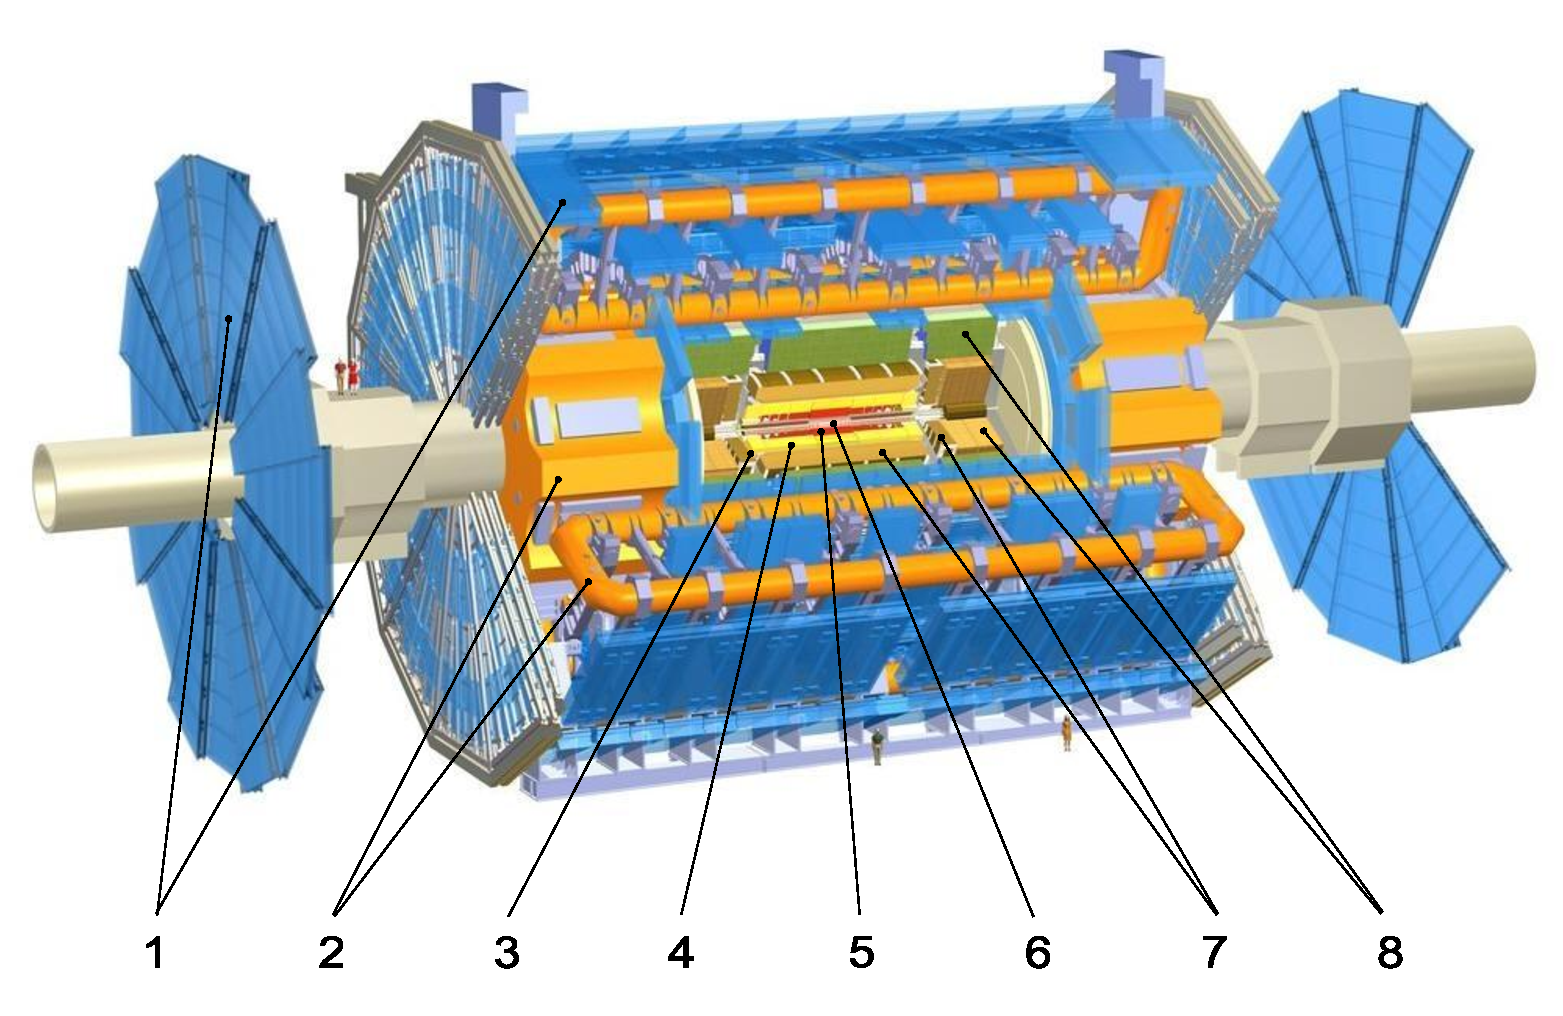
\includegraphics[width=\textwidth]{ATLAS_Drawing_with_Labels.pdf}
    \caption{ATLAS探测器剖面图\cite{ATLAS_detector}}
    \label{fig:ATLAS_Drawing_with_Labels}
    \figurenote{
        μ 子谱仪:
        (1)前向区域(端盖)与筒形区域。
        磁体系统:
        (2)环形磁体,
        (3)螺线管磁体。
        内部径迹探测器:
        (4)穿越辐射探测器,
        (5)硅微条探测器,
        (6)硅像素探测器。
        量能器:
        (7)液氩量能器,
        (8)瓦状量能器(tile calorimeter)。
    }
\end{figure}


\section{内部径迹探测器}
内部径迹探测器(Inner Detector)是 ATLAS 探测器最靠近束流(beam line)探测器系统,
它的主要目的是探测对撞产生的粒子在探测器中的径迹,以确定它们的位置、动量与电荷量。
内部径迹探测器的剖面图见\autoref{fig:Inner_detector},它从内到外主要分为三个部分:
硅像素探测器(Silicon Pixel Detector)、硅微条探测器(Silicon Microstrip Detector)与穿越辐射探测器(Transition Radiation Tracker)。

\begin{figure}[ht]
    \centering
    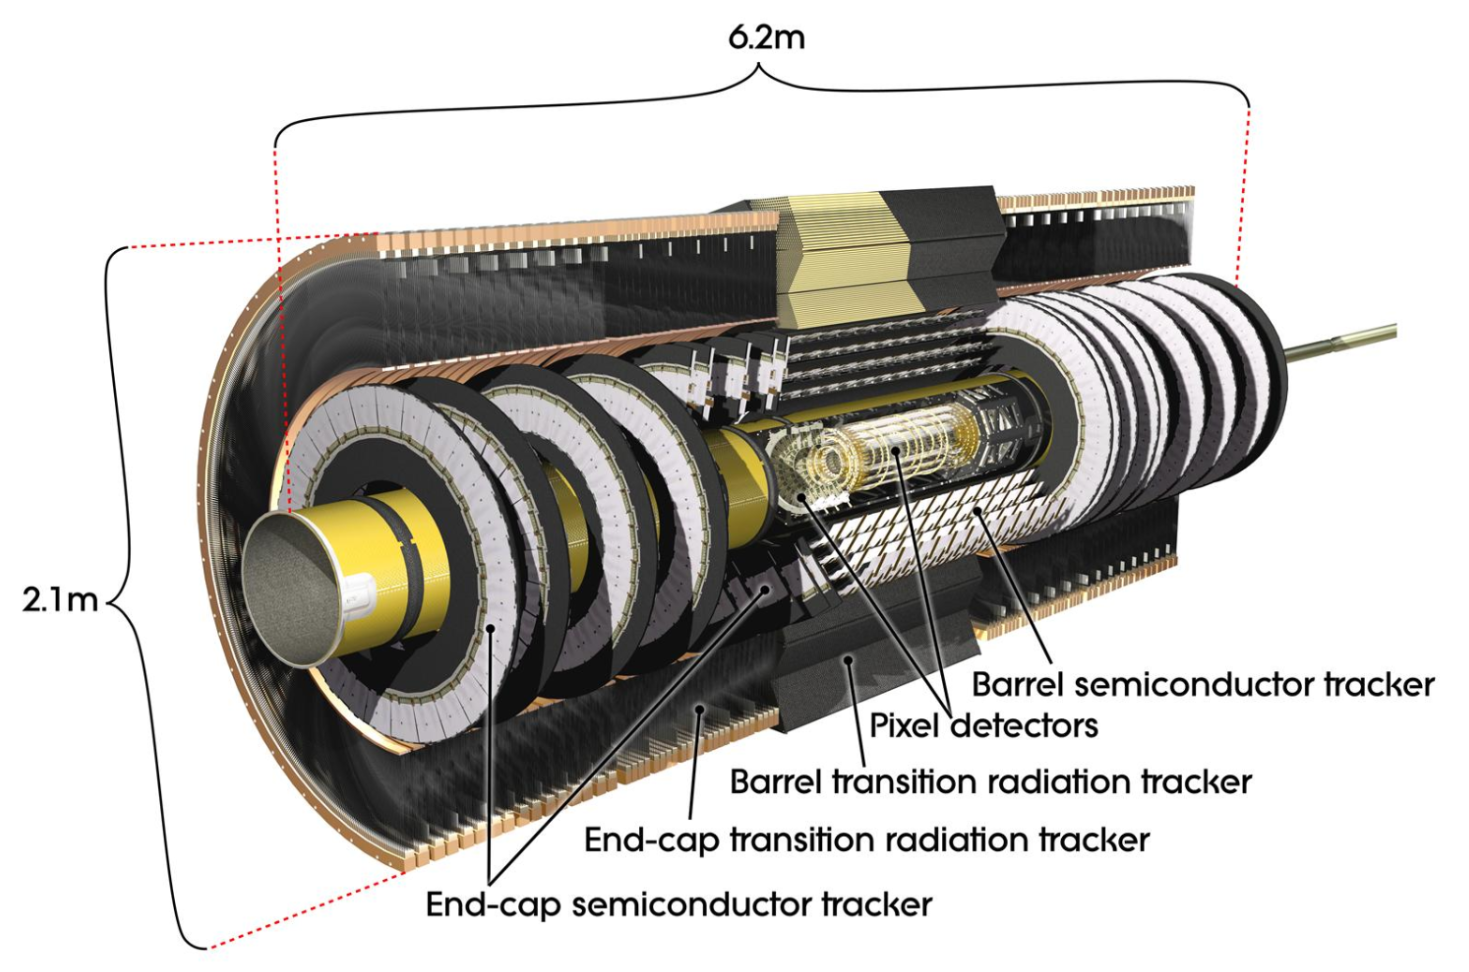
\includegraphics[width=\textwidth]{Inner_detector.png}
    \caption{内部径迹探测器剖面图\cite{ATLAS_detector}}
    \label{fig:Inner_detector}
\end{figure}

高粒度硅像素探测器覆盖顶点区域,筒部为每个径迹提供四次位置测量,用来精确确定作用顶点位置。
像素探测器被硅微条探测器包围,为每条径迹提供四次三维位置测量,用来重建粒子径迹。
这些硅探测器由穿越辐射探测器补充,以获取高能粒子的洛伦兹因子 $\gamma$,用以粒子鉴别。
内部径迹探测器的覆盖范围可达 $\abs{\eta} < 2.5$。


\section{量能器}
量能器通过测量高能粒子在其中发生簇射沉积的能量来直接测量粒子能量。
带电粒子会在电磁量能器(Electromagnetic Calorimeter)中发生电磁簇射,
仅有电磁相互作用的光子与电子一般会在电磁量能器中沉积所有能量,而带电强子只会沉积部分能量。
强子会在强子量能器(Hadronic Calorimeter)中发生强子簇射,由于强子的核作用长度较长,强子量能器通常为取样型。
ATLAS探测器中的量能器覆盖赝快度范围 \( |\eta| < 4.9 \),
主要由液氩(Liquid Argon, LAr)量能器与瓦状强子量能器(Tile Hadronic Calorimeter)组成,
其剖面图见\autoref{fig:Calorimeter}。

\begin{figure}[ht]
    \centering
    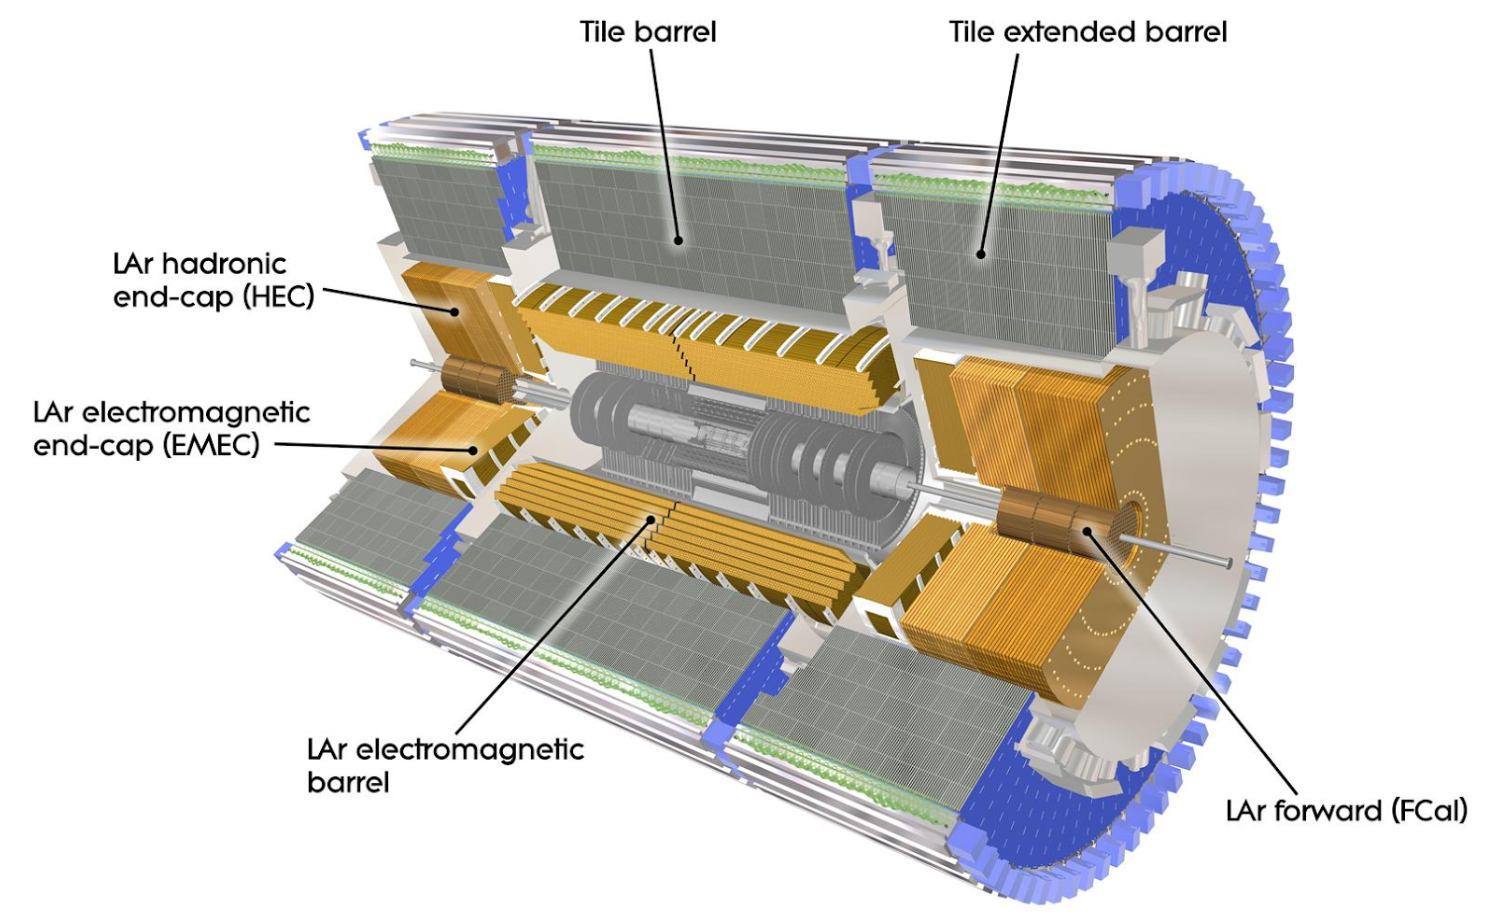
\includegraphics[width=\textwidth]{Calorimeter.png}
    \caption{量能器剖面图\cite{ATLAS_detector}}
    \label{fig:Calorimeter}
\end{figure}

在区域 \( |\eta| < 3.2 \) 内的电磁量能器系统由筒部和端盖的高颗粒度铅、液氩电磁量能器组成,
并在 \( |\eta| < 1.8 \) 范围内配备一个额外的薄层液氩预采样器,用于校正粒子在量能器前方材料中的能量损失。
电磁量能器在筒部的径向距离范围为 \( r = 1.5\,\text{m} \) 到 \( 2.0\,\text{m} \),
在端盖中的轴向位置范围为 \( |z| = 3.6\,\text{m} \) 到 \( 4.25\,\text{m} \)。
强子量能器由钢、闪烁体瓦状量能器构成,在 \( |\eta| < 1.7 \) 的范围内被划分为三个筒状结构,
覆盖径向范围 \( r = 2.25\,\text{m} \) 到 \( 4.25\,\text{m} \)(尽管有效材料仅延伸至 \( 3.9\,\text{m} \))。
此外,在端盖 \( |\eta| > 1.5 \) 的区域由两个铜、液氩强子端盖量能器进行覆盖,
覆盖轴向范围 \( |z| = 4.3\,\text{m} \) 到 \( 6.05\,\text{m} \)。
为了实现完整的立体角覆盖,系统还包括分别针对电磁和强子测量进行了优化的前向铜、液氩与钨、液氩量能器模块。

量能器在轴向与法向都具有高颗粒度。
筒部的量能器总共有七个采样层,包括液氩预采样器、三个电磁量能器和三个强子量能器;
端盖区域提供多达八个采样层,包括预采样器、三个电磁量能器和四个强子量能器。
前向量能器模块在前向区域提供三个采样层。
用于强子能量测量的量能器总深度几乎在整个探测器接受范围内的任何地方都超过九个核作用长度。

由于同时存在筒部与端盖的量能器,下面两个条件之一为确定一个jet为目标CalRatio jet的必要条件:
\begin{itemize}
    \item LLP在筒部衰变:$|\eta|<1.4$且$\SI{0.5}{m}<L_{xy}<\SI{4}{m}$;
    \item LLP在端盖衰变:$|\eta|>1.4$且$\SI{2}{m}<L_{z}<\SI{6}{m}$。
\end{itemize}
其中$L_{xy}$($L_{z}$)为LLP衰变位置在$x$--$y$平面($z$轴)上与探测器中心的距离,
$\eta=-\ln \tan ({\theta}/{2})$为喷注的赝快度。

强子喷注是由经过校准的三维拓扑团簇 (\topos)重建而来。
拓扑团簇是由量能器单元通过拓扑聚类算法组合而成的,这些对象提供了量能器中能量沉积的三维表示。
\cite{Boccardi:1411357}

\section{μ子谱仪}
μ子谱仪用来鉴别 μ 子,并测量它的动量。
μ子谱仪包括单独的触发器和高精度径迹测量室,用于测量超导空心环形线圈产生的磁场中 μ 子的偏转。
环形线圈的场积分在大多数探测器上介于 2.0 到 6.0 Tm 之间。
